In the \wh{} analysis, one of the dominant prompt backgrounds in the \zdom{} and \zdep{} SRs arise from $WZ/W\gamma^{*}$ production. Following the strategy used in the Run~2 analysis, three orthogonal $WZ$ CRs are defined to derive NFs that correct for potential mis-modeling of this background. These CRs use the same selection criteria as the \zdom{} SR, except requiring at least one SFOS lepton pair with an invariant mass within 25~GeV of the $Z$ boson mass. To account for the jet multiplicity dependence observed in Run~2, the control regions are categorized by jet count: a 0-jet CR (WZCR 0j), a 1-jet CR (WZCR 1j), and a 2-or-more jet CR (WZCR 2+j). Figure~\ref{fig:vh_wh_wzcr_numjets} shows the pre-fit data/MC-simulation agreement in each $WZ$ CR, where potential mis-modeling of the background is observed.

\begin{figure}[htp]
  \centering
  \subfloat[$WZ$ 0-jet CR]{
    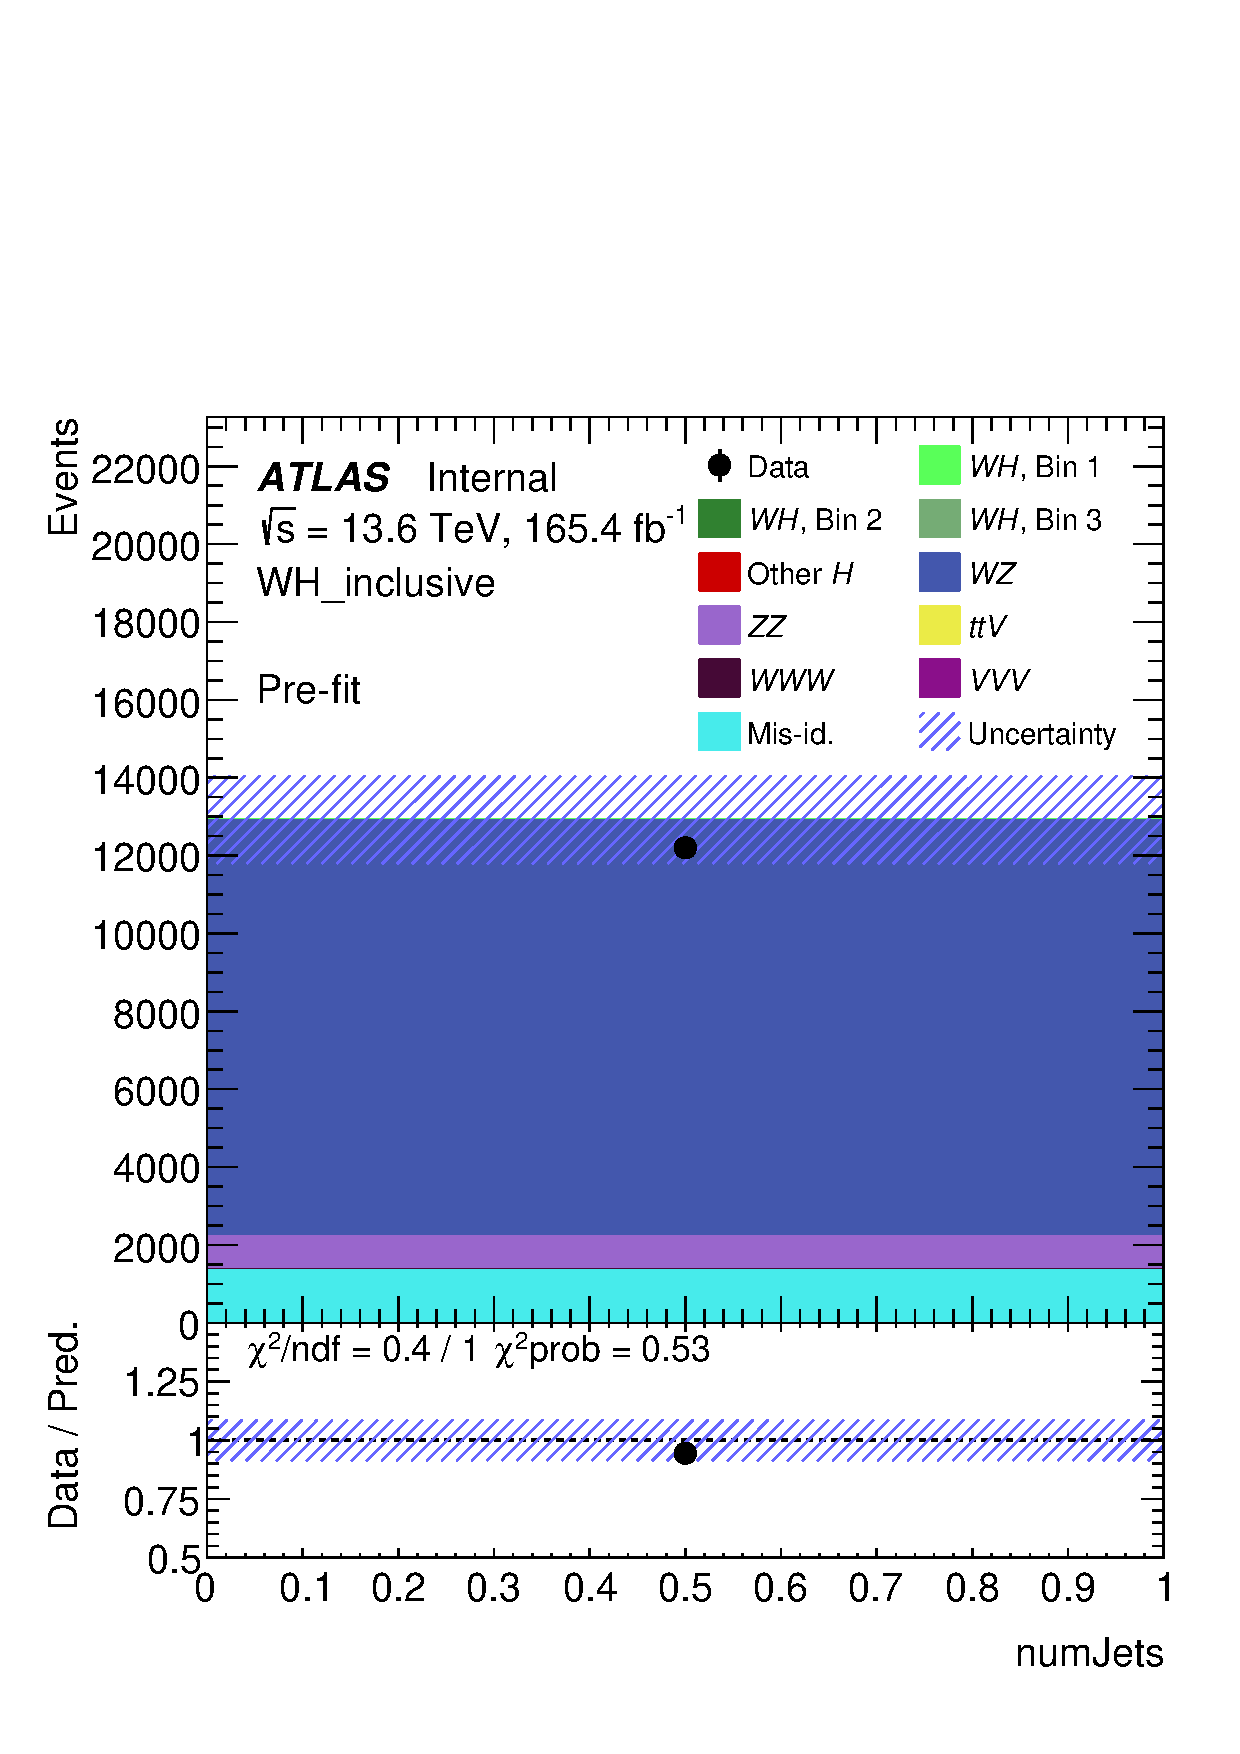
\includegraphics[width=0.45\textwidth]{figures/VH/VH_wzcr_0jet_numjets.pdf}\label{fig:vh_wh_wzcr_0j_numjets}
  }
  \subfloat[$WZ$ 1-jet CR]{
    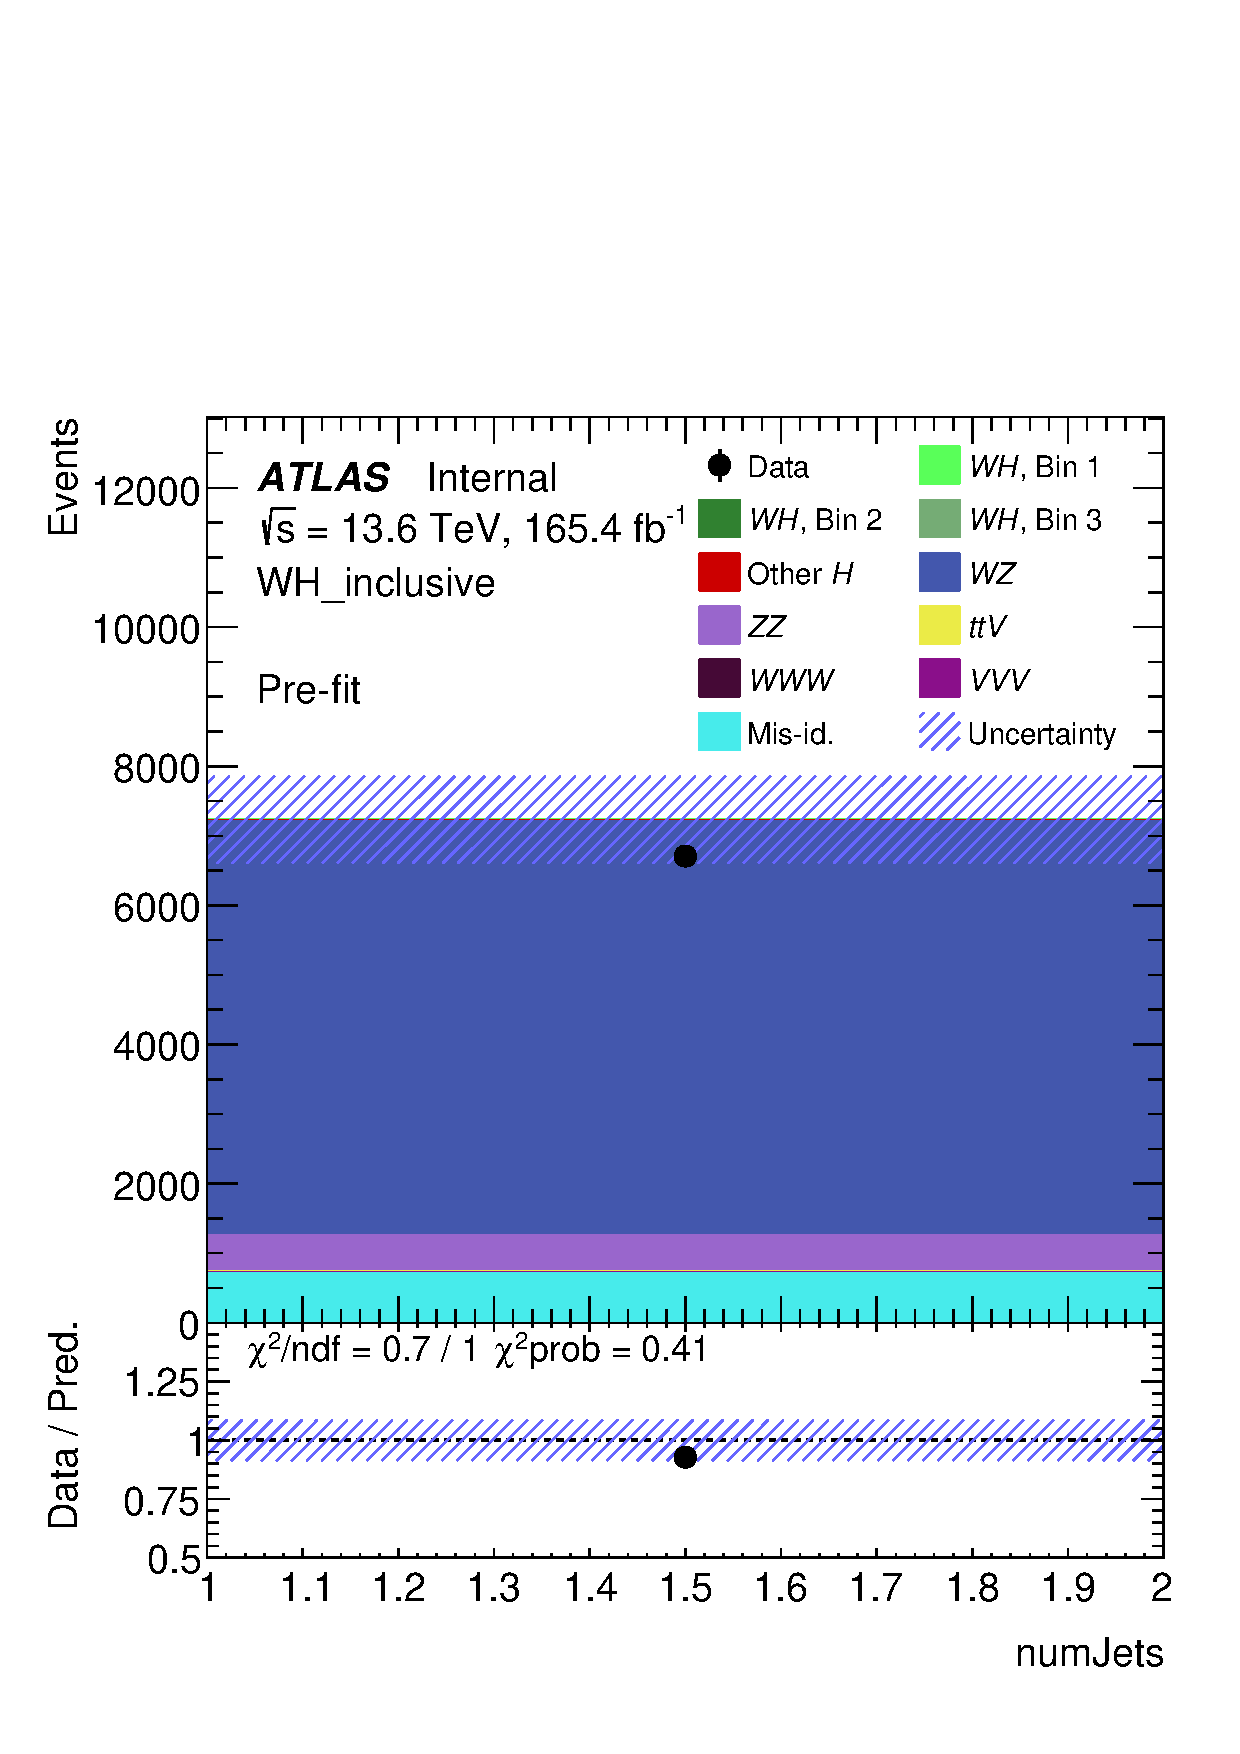
\includegraphics[width=0.45\textwidth]{figures/VH/VH_wzcr_1jet_numjets.pdf}\label{fig:vh_wh_wzcr_1j_numjets}
  }
  \hfill
  \subfloat[$WZ$ 2-or-more jet CR]{
    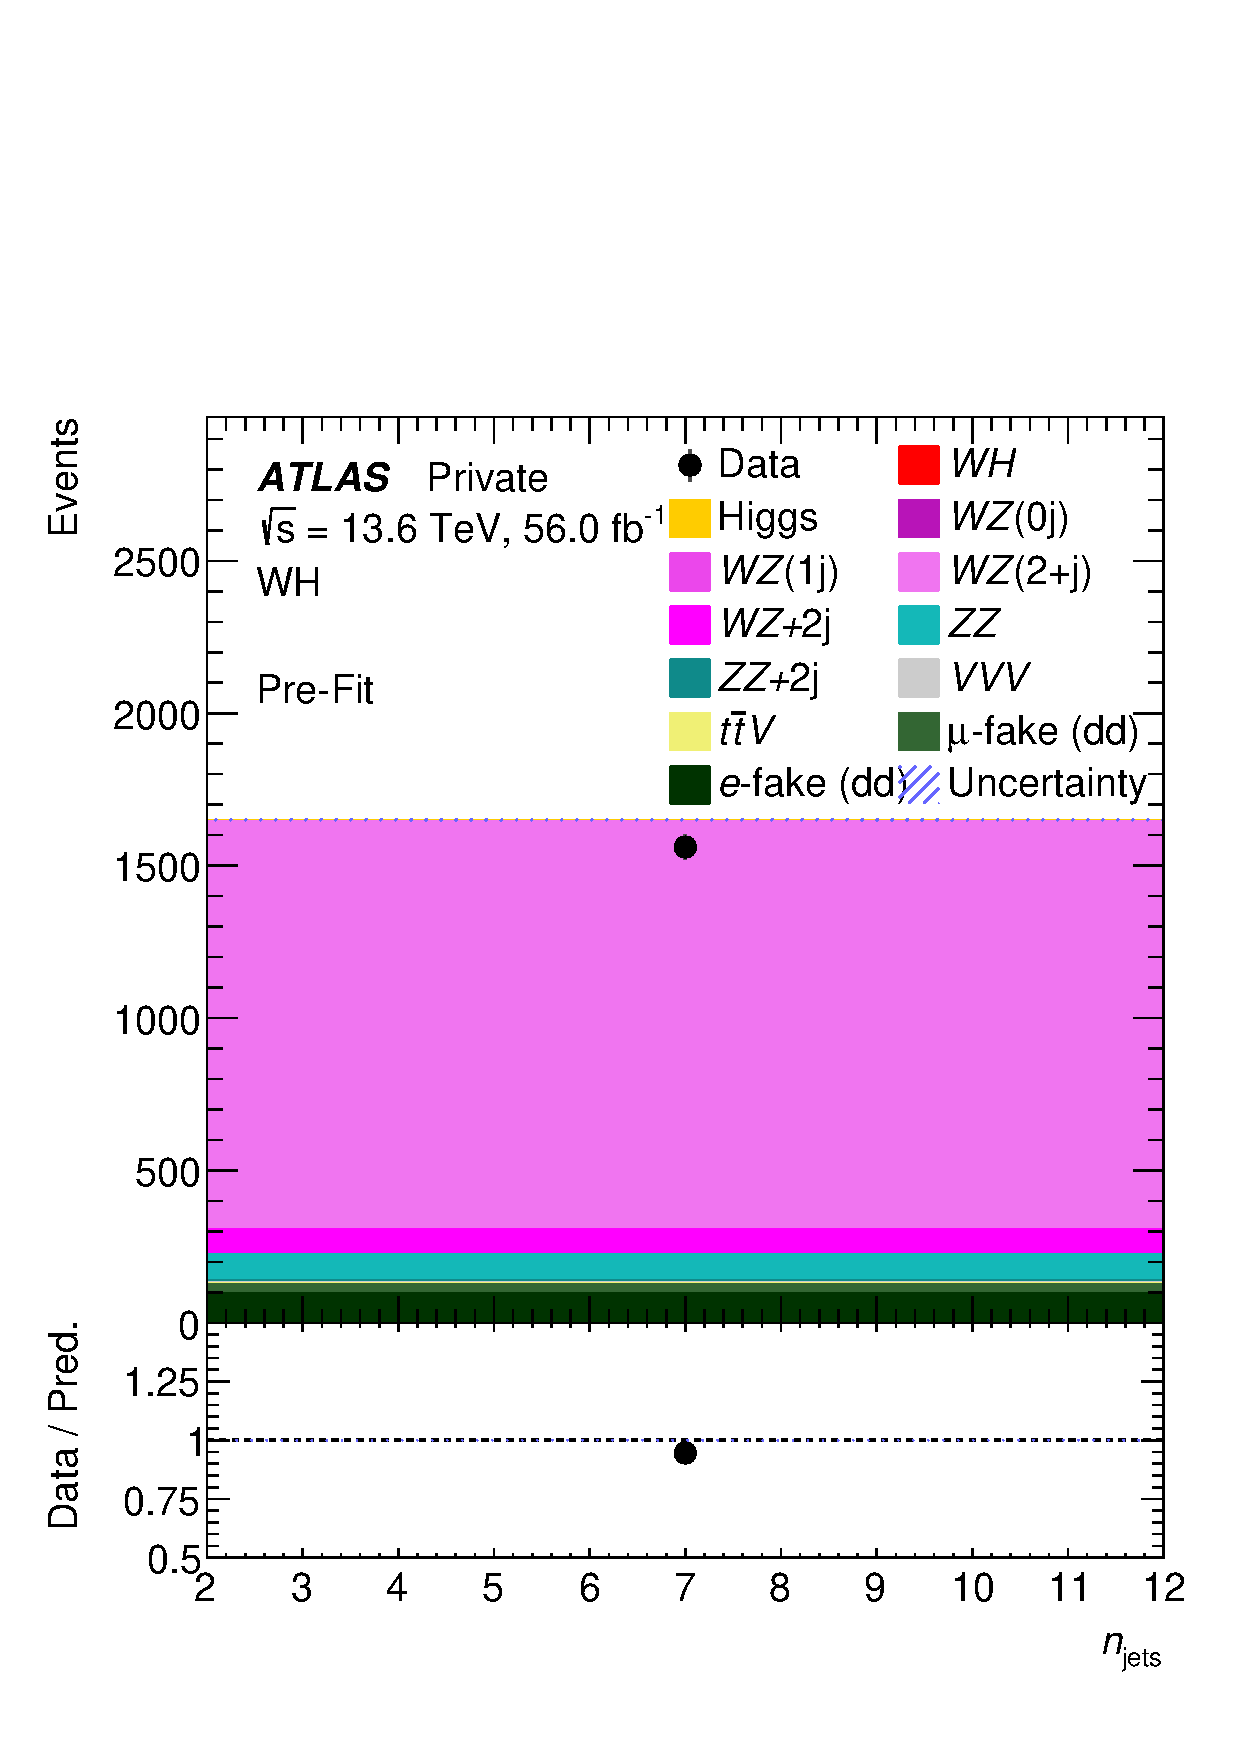
\includegraphics[width=0.45\textwidth]{figures/VH/VH_wzcr_2jet_numjets.pdf}\label{fig:vh_wh_wzcr_2j_numjets}
  }
  \caption{Pre-fit MC/data agreement in the $WZ$ CRs. The $WZ$ 0-jet CR, $WZ$ 1-jet CR, and the $WZ$ 2-or-more jet CR are shown in in (a), (b), and (c) respectively.}\label{fig:vh_wh_wzcr_numjets}
\end{figure}

Following a similar strategy to the Run~2 analysis a dedicated $WWW$ CR is defined to help constrain the $WWW$ background in the final fit due to an excess that was observed previously. This region is defined to be identical to the \zdep{} SR, except requiring all events to have a $WWW$ score $\geq 0.4$. This value was chosen as it provides a region with high $WWW$ purity and low contamination from $WH$. These values are summarized below in Table~\ref{tab:vh_wh_www_cr}.

In Run~2, the on-shell SM $WWW$ analysis measured an excess of events resulting in a signal strength of $\mu=1.61$~\cite{STDM-2019-09}. This was confirmed in the Run~2 $VH$ analysis which measured a NF of 2.07, in agreement with the $WWW$ analysis measurement. A similar excess is observed in the Run~3 iteration of the analysis in the $WWW$ CR. The excess is noticeble in events that have a $WWW$ ANN score between 0.5 and 0.9 as can be seen in Figure~\ref{fig:vh_wh_wwwcr_www_score}.

The normalization factors extracted from these regions are constrained in the statistical analysis as described in Chapter~\ref{ch:statistical_analysis}. Post-fit distributions of the relevant kinematic variables in the $WZ$ CR are shown in Appendix~\ref{app:wzcr_input_plots}, and those for the $WWW$ CR are shown in Appendix~\ref{app:wwwcr_input_plots}.
\begin{figure}[htp]
    \centering
    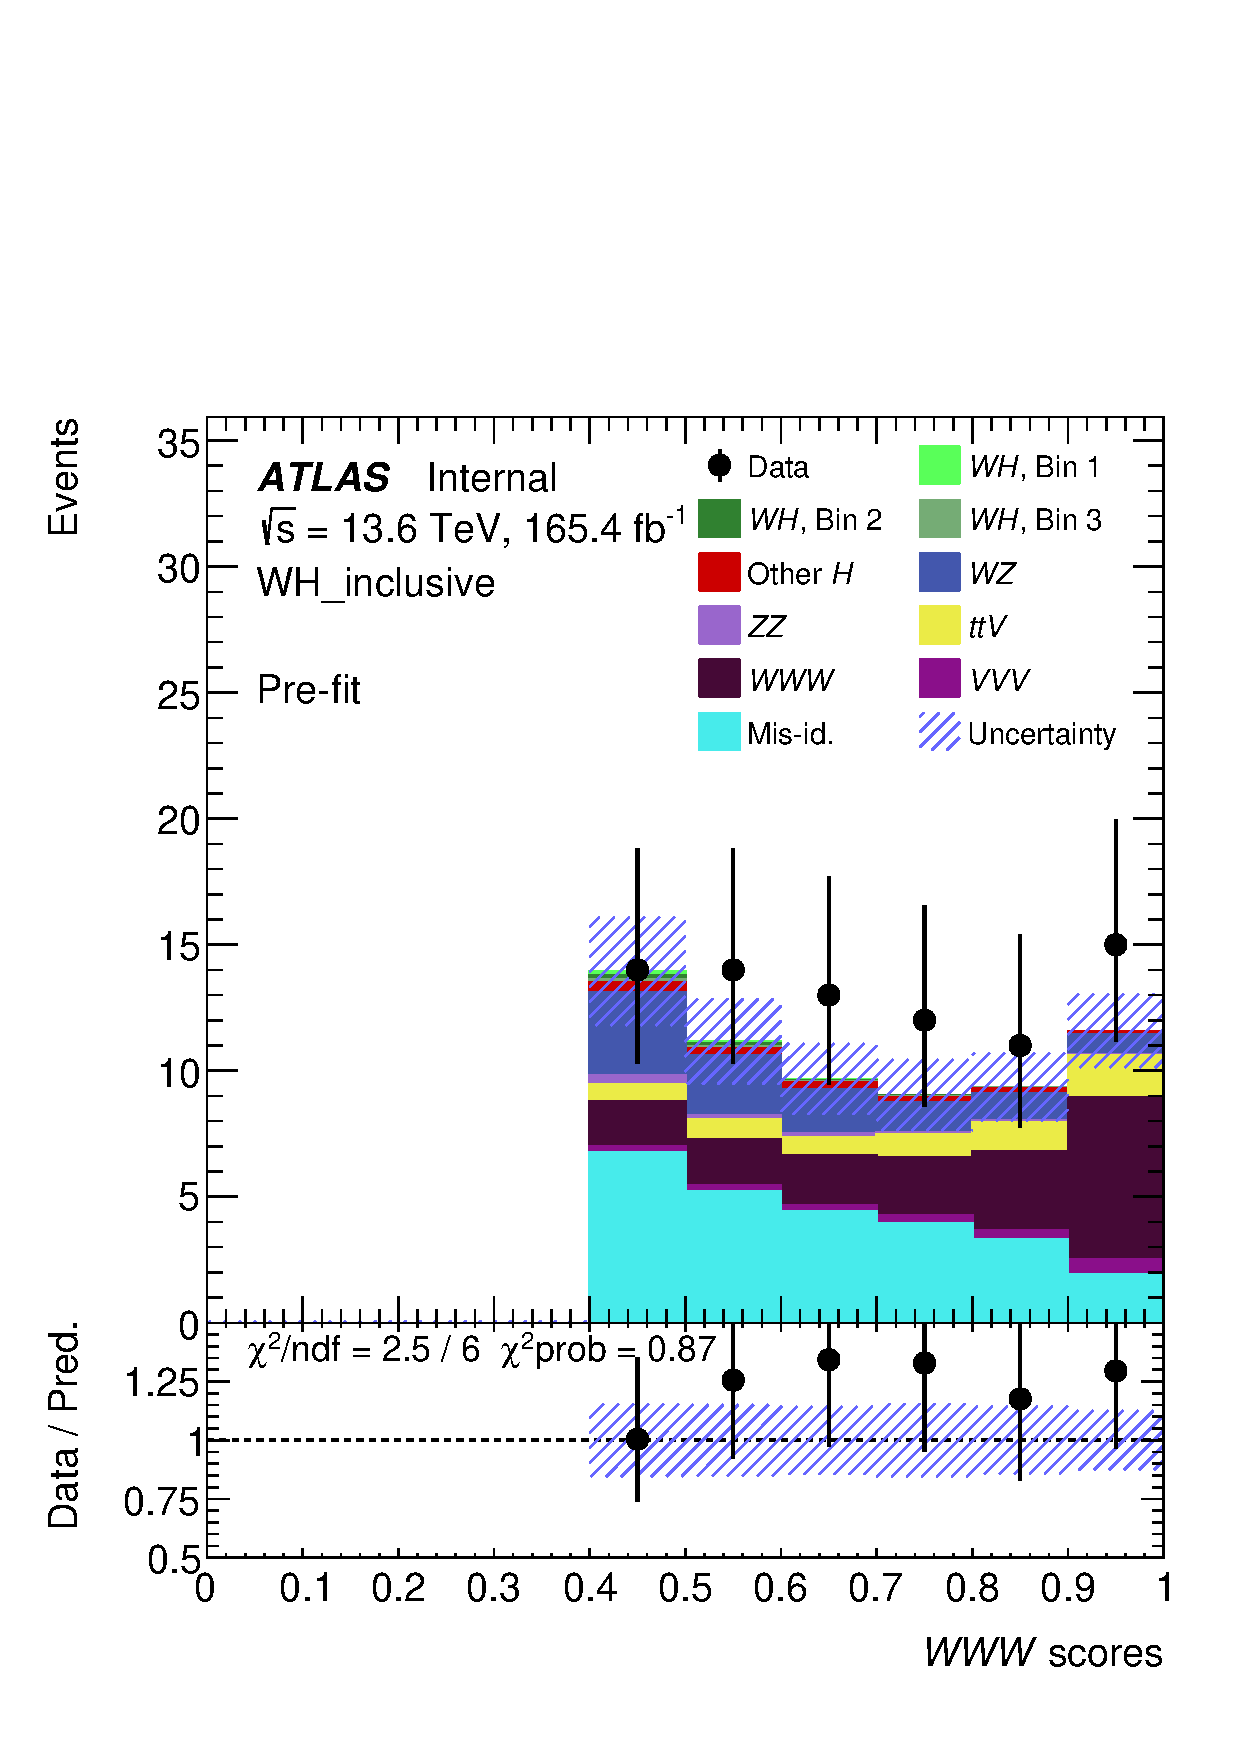
\includegraphics[width=0.5\textwidth]{figures/VH/VH_wwwcr_www_scores.pdf}
    \caption{Pre-fit data/MC-simulation agreement in the $WWW$ CR. A clear excess of events is seen in the $WWW$ output node when the $WWW$ score is greater than 0.5.}\label{fig:vh_wh_wwwcr_www_score}
\end{figure}

\begin{table}[htp]
    \centering
    \resizebox{1\textwidth}{!}{
    \begin{tabular}{c||c|c|c|c|c}
        \hline
        \text{$WWW$ Score Cut} & \text{$WH$ Yield} & \text{$WWW$ Yield} & \text{Total Yield} & \text{$WH$ Contribution} & \text{$WWW$ Purity} \\
        \hline
        \text{$\geq$ 0.0} & 18.5  & 27.2 & 273   & 6.78\% & 9.97\% \\
        \text{$\geq$ 0.1} & 9.52  & 25.0 & 168   & 5.68\% & 14.9\% \\
        \text{$\geq$ 0.2} & 3.42  & 21.8 & 103   & 3.31\% & 21.0\% \\
        \text{$\geq$ 0.3} & 1.67  & 19.4 & 75.9  & 2.20\% & 25.6\% \\
        \text{$\geq$ 0.4} & 0.90  & 17.5 & 59.0  & 1.53\% & 29.7\% \\
        \text{$\geq$ 0.5} & 0.50  & 15.7 & 45.1  & 1.11\% & 34.8\% \\
        \text{$\geq$ 0.6} & 0.26  & 13.8 & 35.5  & 0.73\% & 39.0\% \\
        \text{$\geq$ 0.7} & 0.13  & 11.9 & 27.1  & 0.48\% & 43.7\% \\
        \text{$\geq$ 0.8} & 0.05  & 9.55 & 19.3  & 0.26\% & 49.5\% \\
        \text{$\geq$ 0.9} & 0.01  & 6.43 & 11.0  & 0.09\% & 58.6\% \\
    \end{tabular}
    }
    \caption{Event yields in the Z-depleted SR from simulation as a function of minimum $WWW$ ANN output node score. The $WH$ signal and $WWW$ fractions are also provided. }\label{tab:vh_wh_www_cr}
\end{table}